\documentclass[a4,center,fleqn]{NAR}
\usepackage{hyperref}
\usepackage{graphicx}
\usepackage{csquotes}
\usepackage{amsmath}
\usepackage{setspace}
\usepackage{float}
\usepackage{caption}
\usepackage{subcaption}
\usepackage[super]{nth}
\usepackage{multirow}
% Enter dates of publication
\copyrightyear{2017}
\pubdate{18 March 2017}
\pubyear{2017}
\jvolume{37}
\jissue{12}

\usepackage{tikz}
\usetikzlibrary{shapes}
\usetikzlibrary{positioning}
\usetikzlibrary{arrows}
\usetikzlibrary{fit}
\usetikzlibrary{decorations.pathreplacing}
\usetikzlibrary{shadows.blur}
\usetikzlibrary{shapes.symbols}

%\articlesubtype{This is the article type (optional)}

\begin{document}
\title{HiC Contact Map Comaprison Using Graphlet Approach}

\author{%
    Behnam Rasoolian\,$^{1,*}$,
    Debswapna Bhattacharya\,$^{1}$
    \footnote{
    Tel: +1 334 5212814; Email: bzr0014@auburn.edu}}

    \address{%
        $^{1}$ Auburn University
        }
        % Affiliation must include:
        % Department name, institution name, full road and district address,
        % state, Zip or postal code, country

%        \history{%
%            Received January 1, 2009;
%            Revised February 1, 2009;
%            Accepted March 1, 2009}

            \maketitle

\begin{abstract}
    Chromosal Conformational Capturing (3C) data,
    particularly the Hi-C data is widely used for
    investigating the three-dimensional (3D) 
    chromatin conformation inside the nucleus and
    for identifying chromatin interactions as 
    well as topologically associating domains 
    (TADs). However, Hi-C based structural analysis
    for exploring local chromatin conformational 
    preferences has not been performed yet. 
    Here, for the first time, we present graphlet
    based local structural analysis for normal 
    and malignant human cell types  using chromosal
    conformational capturing (Hi-C) data. 
    We first applied thresholding in Hi-C interaction
    frequency data for one normal cell line and 
    four leukemic cells lines in order to covert 
    them into unweighted graphs. We then mined 
    the unweighted graphs to extract graphlet -based 
    orbitial frequency distributions? . Subsequently
    , pairwise graphlet distances as well as 
    pairwise graphlet distribution correlations 
    for each pair of cells were computed and 
    compared using statistical methods namely 
    ANOVA and multi-variate ANOVA. Our results 
    demonstrate that normal-cancer pairs have 
    significantly ($F(1, 1654) = 20.49$, $p-value
    < 0.0001$) higher difference than cancer-cancer 
    pairs. Furthermore, for certain orbits cancer-cancer 
    pairs demonstrated higher correlations 
    ($F(365, 7882)=391$, $p-value<0.00001$, and 
    $Wilk's \quad \Lambda=0456$) than normal-cancer pairs 
    in terms of orbit frequency distributions. 
    Source code of GrapHiClet 
    is freely available at 
    \url{https://github.com/rasoolianbehnam/watson}.
    Also, the database used for this project can be
    found at \url{https://graphiclet.localtunnel.me/secret/}
\end{abstract}

\section{Introduction}
Genome of a eukaryotic cell is organized into a
complex three-dimensional (3D) structure, which
leads to a network of chromosomal interactions \cite{dekker2008gene}.
The spatial organization of genome is one of
the most important factors in determining its
function \cite{fraser2007nuclear} via interactions between
spatially close genes \cite{kagey2010mediator}. Such
interactions can be modeled using a network approach
\cite{kagey2010mediator}. However, our knowledge of
3D conformation of genome is limited. Fluorescent In
Situ Hybridization (FISH) technology, which can
capture 3D conformation of multiple loci but cannot
capture global layout of the genome. In order to
address this, more advanced techniques of chromosome
conformation capturing such as 3C \cite{dekker2002capturing},
4C \cite{simonis2006nuclear} and 5C \cite{dostie2007mapping}
has been introduced which are based on chromatin fragment
fixation, using restriction-enzyme digestion and
intra-molecular ligation. One of the most recent
versions of chromosome conformation capturing is
Hi-C \cite{rao20143d, lieberman2009comprehensive},
which $IF_{ij}$ captures interactions between chromosomal
fragments resulting in a contact map or interaction frequency
(IF) matrix, which captures the number of interactions
detected in Hi-C dataset between each pair of loci.

Recently, Hi-C data has been mostly used to predict
the 3D structure at the chromosome level by satisfying
intra-chromosomal interactions or even at the
full genome by leveraging both inter- and intra-chromosomal
interactions
\cite{noble2011three, 
rousseau2011three, 
hu2013bayesian, 
varoquaux2014statistical, 
trieu2014large, 
zhang20133d, 
lesne20143d, 
bau2011three, 
adhikari2016chromosome3d}.
These efforts, although different in
approach, usually translate interaction frequencies in
contact maps as simple inverse measures of distance.
They then try to find the coordinates of the chromosomal
loci that would result in that particular distance
matrix using optimization. These methods vary in
the optimization models and methodologies used.
Also, efforts has been made recently to learn the
inverse conversion parameters from contact maps
to distance matrices \cite{oluwadare2018maximum}.
The reconstructed 3D structures could be used in
order to compare normal and malignant cell lines.
However, the main obstacle to doing so is that
the process of reconstruction is computationally expensive.
Almost all reconstruction methods rely on either
deterministic or heuristic optimization approaches in
order to find the best conformation that matches contact
maps. Also, there is no experimental way of evaluating
the accuracy of the reconstructed 3D conformations.
One experimental way of partially validating correctness
of reconstruction process is Fluorescence in
situ hybridizaiton (FISH) method. However, this
technique is limited to a few loci and cannot be
extended to cover the whole structure of the chromosomes.
Furthermore, the process of reconstructing 3D
chromatic structure is computationally expensive,
hindering their applicability at the genome-wide scale.
% **************************************************************
% Keep this command to avoid text of first page running into the
% first page footnotes
\enlargethispage{-65.1pt}
% **************************************************************


Over the past decade, graphs have been used extensively
in order to model domain-specific phenomena such
as computer security, gene regulatory networks and
social networks. These graphs are usually in
the form of very large networks. It is often necessary
to perform statistical analysis between graphs in
order to compare their structure. Graphlets and
orbits can be used in order to probe large graphs
in order to find global and local similarities 
\cite{shervashidze2009efficient, borgs2006counting,
bondy1977graph}.
This can be done by counting the number of occurrences
of a each graphlet and/or orbits for each node
in the whole graph and the comparing them \cite{prvzulj2007biological,
prvzulj2004modeling}

Here, we present local structural analysis between
4 sets of Hi-C data. All four data sets are sequences
from the same cell line, with one of them being
a normal cell and the other three sequenced from
three types of leukemic cells. In order to achieve
this, we used graphlets, given their strength in
capturing information about local structures of
a graph. We first thresholded Hi-C interaction frequency
matrices in order to convert in to an unweighted undirected
graph adjacency matrix. We the extracted counts of
the first 73 orbits for each node, identifying each
node with a signature vector of size 73. We then
applied graphlet distance metrics proposed in
\cite{prvzulj2007biological} together with statistical methods
in order to find difference between cell lines.
Our results show that difference of local structure
between normal cells and leukemic cells are significantly
larger that difference between cancer-cancer cells.  

\subsubsection{Notations}
%In this paper, matrices and vectors are represented using bold
%capital and bold small letters respectively.
%Matrix rows and columns are represented by a \textit{dot}
%notation. For example, the $i$th row of matrix $M$ is
%denoted by $M_{i.}$ and its $j$th column is represented
%by $M_{.j}$.

We denote the set of all contact maps in cell line $K$ with 
$\mathbb{C}^K$. If no particular cell line is addressed, the
subscripts are dropped.
Any arbitrary member of $\mathbb{C}$ is denoted by 
$\mathbf{C}_{ij}$, where $i$ and $j$ ($j \ge i$) 
represent the two chromosomes involved. 
In human cells this set contains a total of 276 contact maps,
23 of which are intra-chromosomal and the rest are inter-chromosomal.
For ease of representations, intra-chromosomal contact maps are
distinguished by a single superscript, so we have $\mathbf{C}_{i,i} =
\mathbf{C}_i$.

We denote the number of loci in a chromosome $i$ by $N_i$.
The set of all loci involved in contact map $C_{ij}$ is denoted 
by $\mathbb{V}_{ij}$.
In intra-chromosomal contact maps, $\mathbb{V}_{i,i}$ containts only the 
loci of that particular chromosome ($|\mathbb{V}_i| = N_i$), while in 
inter-chromosomal contact maps $\mathbb{V}_{ij}$ contains the loci in
the both of chromosomes involved 
($\mathbb{V}_{ij} = \mathbb{V}_i \cup \mathbb{V}_j$).


\section{Materials and Methods}
Chromosomes inside the nuclei are made up of
pairs of nucleotides called a base. As a result of
the Hi-C process, a database is generated which
provides interaction counts found by the method between
a number of such bases. The minimum number of
bases that can be captured is called the resolution of
that database. These counts are then binned so
that counts are aggregated for every equal-sized
length of the chromosome (e.g. 1 Mb pairs) leading
to an N * N interaction frequency matrix. Each
cell (i, j) in the matrix is the aggregate count
of all interactions found between loci i\textsuperscript{th} and
j\textsuperscript{th} length.
We re-used Leukemic Hi-C libraries created in
\cite{wang2013properties}. These libraries were sequenced
using Illumina HiSeq 2000 for cases of primary human
B-acute lymphoblastic leukemia (B-ALL or ALL),
the MHH-CALL-4 B-ALL cell line (CALL4), and the
follicular lymphoma cell-line (RL) for which high-quality
paired-end reados of 39M, 79M and 33M were obtained
respectively As in \cite{wang2013properties}, We used
normal B-cell line (GM068990) from as benchmark for
our comparisons. The three datasets generated in
\cite{wang2013properties} were valid since 98\% of
the contact generated in \cite{wang2013properties}
were identical to that of \cite{lieberman2009comprehensive}
and 83\% of contacts in \cite{lieberman2009comprehensive}
were also present in \cite{wang2013properties}. We
created contact maps with bin sizes of  500 kilo-base
and normalized them using normalization provided 
HiC-Pro( \texttt{iced} package in python) developed
by \cite{servant2015hic}.
Normalization is necessary since Hi-C data usually
contains different biases due to GC content,
mappability and effective fragment length \cite{yaffe2011probabilistic,
hu2012hicnorm}. The normalization proivdedi in
the iced package is based on the Sinkhorn-Knopp
algorithm which is a simple, parameter-free and
capability to correct unknown biases.  The edges
in a network usually include indirect dependencies because
correlations are transitive; that is, if there is
a strong realationship between nodes 1 and 2,
and also a strong realationship between nodes 2
and 3, it is highly likely that nodes relationship between
nodes 1 and 3 is exaggerated in the network \cite{feizi2013network}.
In order to remove the effect of indirect interactions,
We also performed and extra normalization by
performing network deconvolution \cite{feizi2013network},
which uses eigenvalue decomposition and infinite series
sums in order to reverse the bias posed by indirect
relationships.

\subsection{Graphlets and Orbits}
\begin{figure}[H]
    \centering
    \includegraphics[width=.5\textwidth]{figures/graphlets.jpg}
    %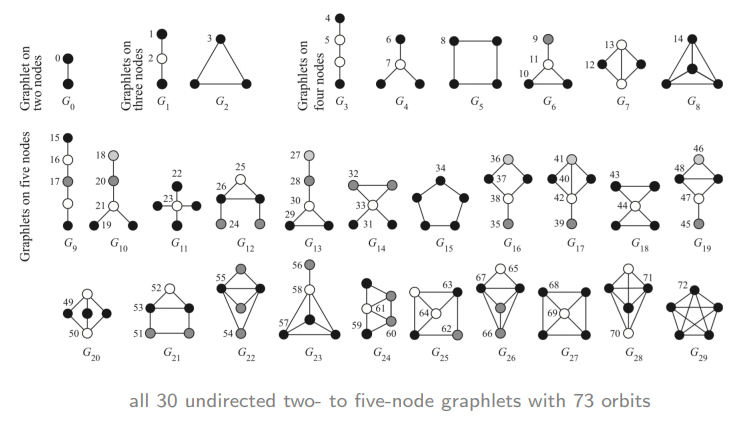
\includegraphics[width=.5\textwidth]{/home/bzr0014/Dropbox/graphlets.png}
    %\includegraphics[width=.5\textwidth]{/home/bzr0014/Dropbox/graphlets.jpg}
    \caption{}
    \label{fig_graphlets}
\end{figure}
Recently, graphlet comparison has emerged as
a novel method for comparing large networks in
order to find local similarities in them. A
graph G is a pair $(V,E)$, where $V$ is a set of
vertices and $E \subseteq V\times V$ is a set of
edges. A connected graph is one where there is
a path between every pair of vertices.
Given a graph $G(V, E)$ and $S \subseteq V$,
then $G'(S, E')$ is a graphlet if and only if
it is connected $E' = \{(u, v) | u, v \in V \quad \&
\quad (u, v) \in E \rightarrow (u, v) \in E'\}$. 
There a total of 30 graphlets
of size 2, 3, and 5.  Figure \ref{fig_graphlets}
demonstrates these graphlets. 
As can be seen there is only one graphlet
of size 2 which is equivalent to an edge; that
is, the number of graphlet 1 in a graph is the
same as the number of edges on the graph. There
are also a total of 2 graphlets of size 2, 6
of size 4 and 20 of size 5. The nodes of each graphlet
can be partitioned into sets of topographically equivalent
nodes called orbits. For  example, in  Figure 
\ref{fig_graphlets}, we can see that G3 can be
partitioned into 2 sets of nodes, the middle ones
(white) and the outer nodes (black). 
For the same set of graphlets,
there are 73 orbits that are also illustrated in
figure  Figure using nodes of difference shades.

\subsection{Thresholding contact maps}
In order to be able to extract graphlets, HiC contact maps should be modeled as
unweighted graphs where the nodes represent the loci and an edge between two 
nodes represent a \textit{significant} interaction between the loci.
This can be achieved by thresholding the contact maps. The result
of the thresholding procedure is a binary matrix which also can serve as
an adjacency matrix for an unweighted, undirected graph. The graph can then be
used for orbit extraction.

When thresholding contact maps, it is necessary to
make sure that both global and local features are
maintained. We could consider thresholding the
contact maps by simply setting values above a
fixed value to one and the rest to zero; However,
in practice, this method resulted in graphs that
capture the local structure of the contact maps
poorly. This is because intensities follow an
exponential distribution with a mean close to
zero with a few very larges values that correspond to
interactions along or close to the main diagonal of
the contact maps.  Thus, picking relatively large
numbers would result in ignoring interactions that
are far from the main diagonal while picking small
values will lead to capturing too many (insignificant)
interactions.

To the best of our knowledge, little work has
dealt with the task of thresholding HiC contact maps.
There has been some statistical approaches developed
on similar data in other fields.  For example,
authors of \cite{ginestet2011statistical} developed
Statistical Network (SPN) analysis where the
choice of thresholding value is made by statistical inference.
This method, although very robust, works within
the framework of design of experiments where the
same network can be extracted for different individuals
under different treatments. Thus a relatively large
set of different contact maps need to be available
in order for this method to be applicable towards
our end.

Instead, in order to threshold the matrix so that both global and local patterns are
captured, we borrowed the concept of \textit{adaptive thresholding} from image 
processing context. In this method, in order to be set, a pixel should have
an intensity larger than the average of non-zero intensities in its
\textit{neighborhood}. The neighborhood is defined by a sliding kernel 
that passes through the contact map with the pixel at its middle at 
each step. Figure \ref{local_thresholded_chr1_chr1} demonstrates result of 
this thresholding approach for intra-chromosomal contact maps of chromosome 1.
Refer to supplementary material for all 23 interchromosomal thresholding
results.
\begin{figure}[t]
    \centering
    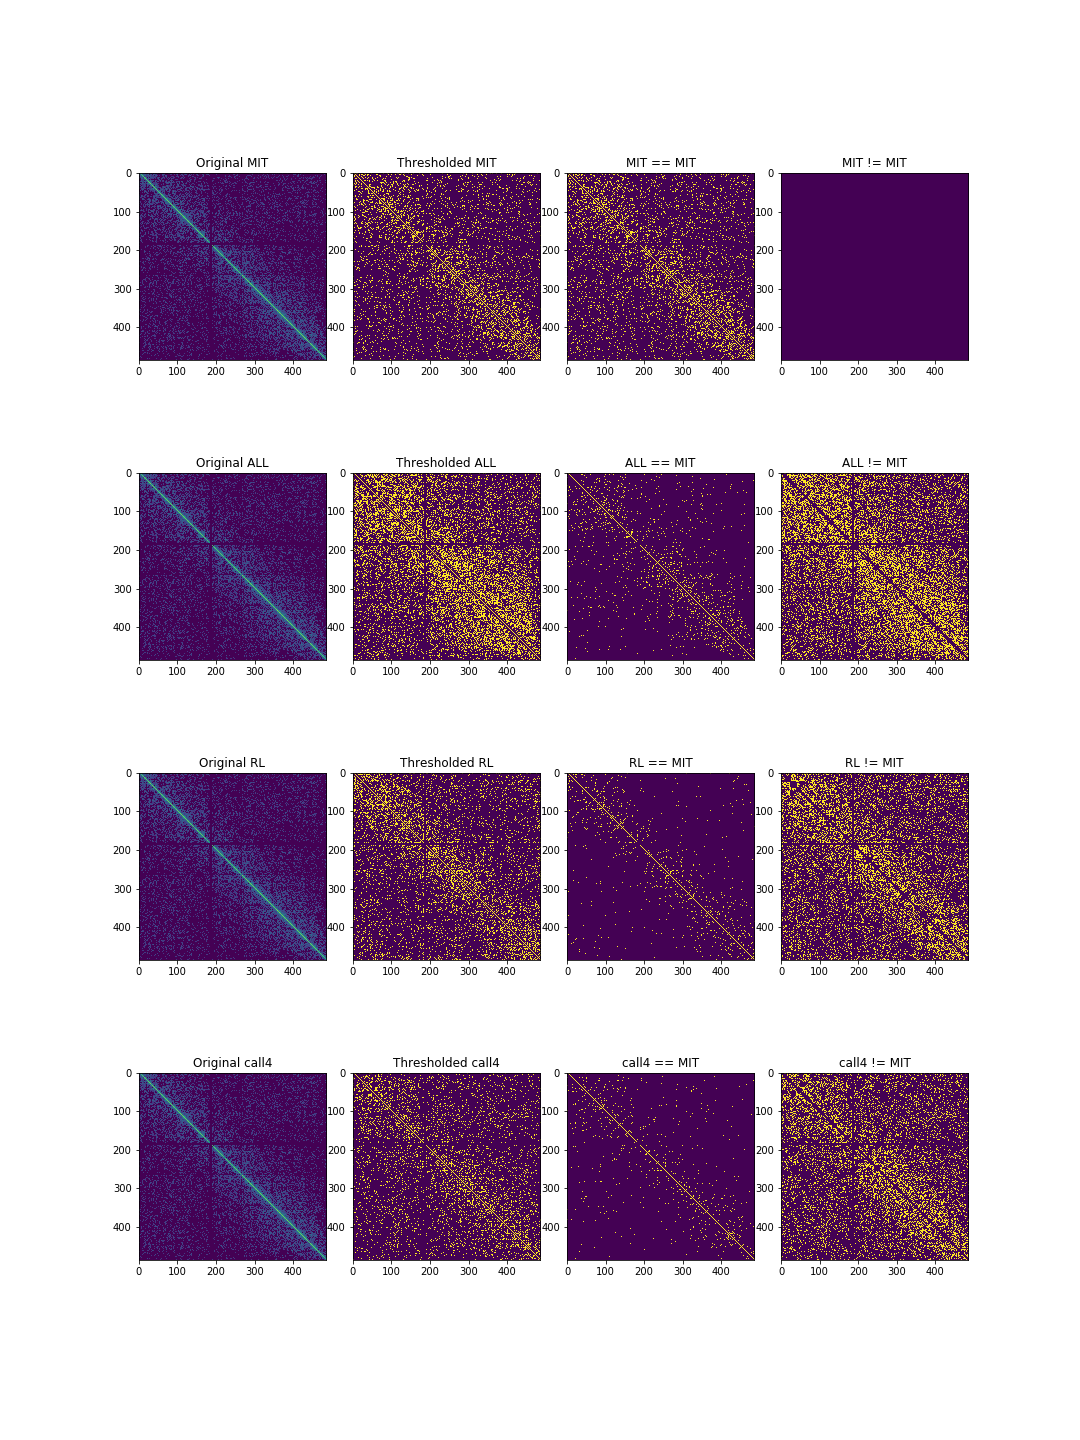
\includegraphics[width=.47\textwidth]{figures/local_thresholded_chr1_chr1.png}
    \caption{Result of thresholding interchromosomal contact map of chromosome 1
    using a kernels of size $5 \times 5$ for all cell lines. 
    The first row shows the thresholded
    maps. Second and third rows demonstrate pair-wise similarities and 
    differences between contact maps respectively.}
    \label{local_thresholded_chr1_chr1}
\end{figure}

\subsection{Orbit Extraction}
Once the thresholded contact maps are obtained, graphlets and orbits can be 
extracted. We used the \texttt{orca} package in \texttt{R} programming 
language to extract the graphlets. As a result of graphlet extraction, 
For each loci in each contact map, a \textit{signature vector} of size
73 is created. Thus for each cell line, we would have 276 
\textit{signature matrices} of
size $|V^{ij}|\times 73$, where $V^{ij}$ is the number of loci
involved in contact map between chromosomes $i$ and $j$. Figure
\ref{fig:graphlet_extraction} illustrates the process and results
of signature matrix extraction schematically.
\begin{figure}
    \centering
    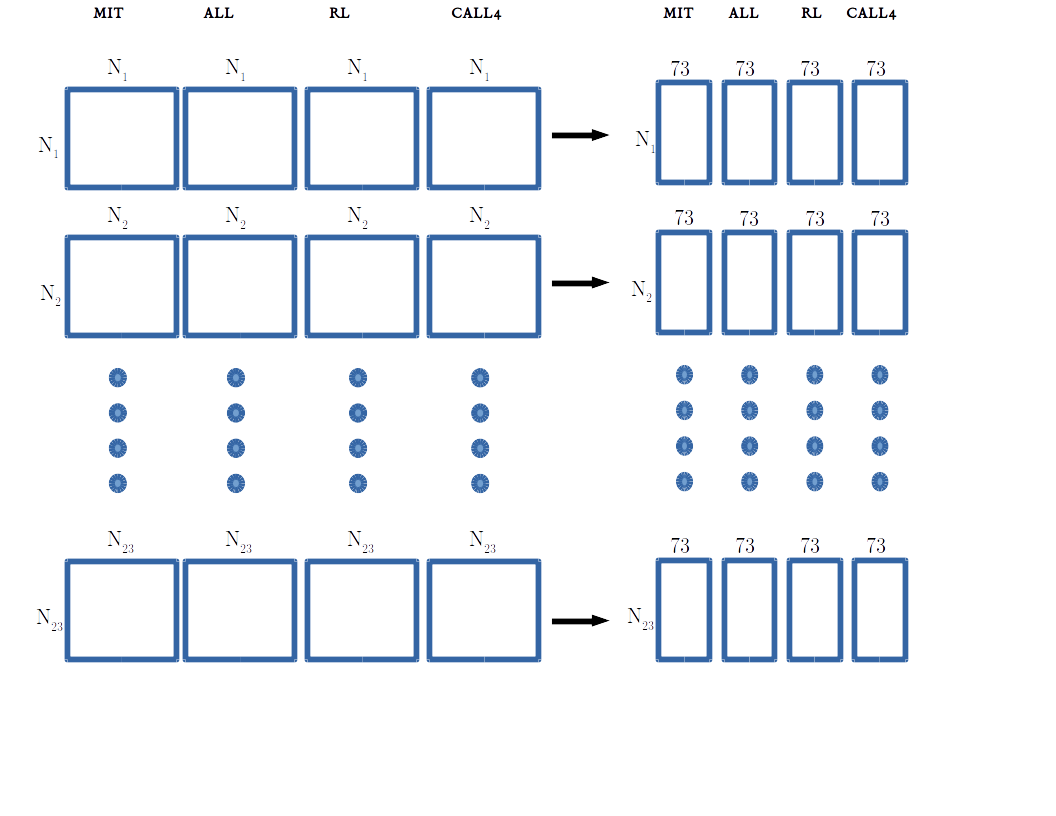
\includegraphics[width=.47\textwidth]{figures/graphlet_extraction.png}
    \caption{Graphlet extraction for the four cell lines. For each
    loci in each contact map between chromosomes $i$ and $j$, 
    the signature vectors of length 73 are extracted, resulting 
    in a \textit{signature matrix} of size $|V^{ij}| \times 73$,
    where $V^{ij}$ 
    is the number of loci involved.}
    \label{fig:graphlet_extraction}
\end{figure}

For a particular
$\mathbf{C}_{ij}$, we denote $\mathbf{S}_{ij}$ as its \textit{signature 
matrix}. Each cell $S_{ijlo}$ in $\mathbf{S}_{ij}$ captures how many
times loci $l$ in $\mathbf{C}_{ij}$ occured as part of orbit $o$.


\begin{figure}
    \centering
    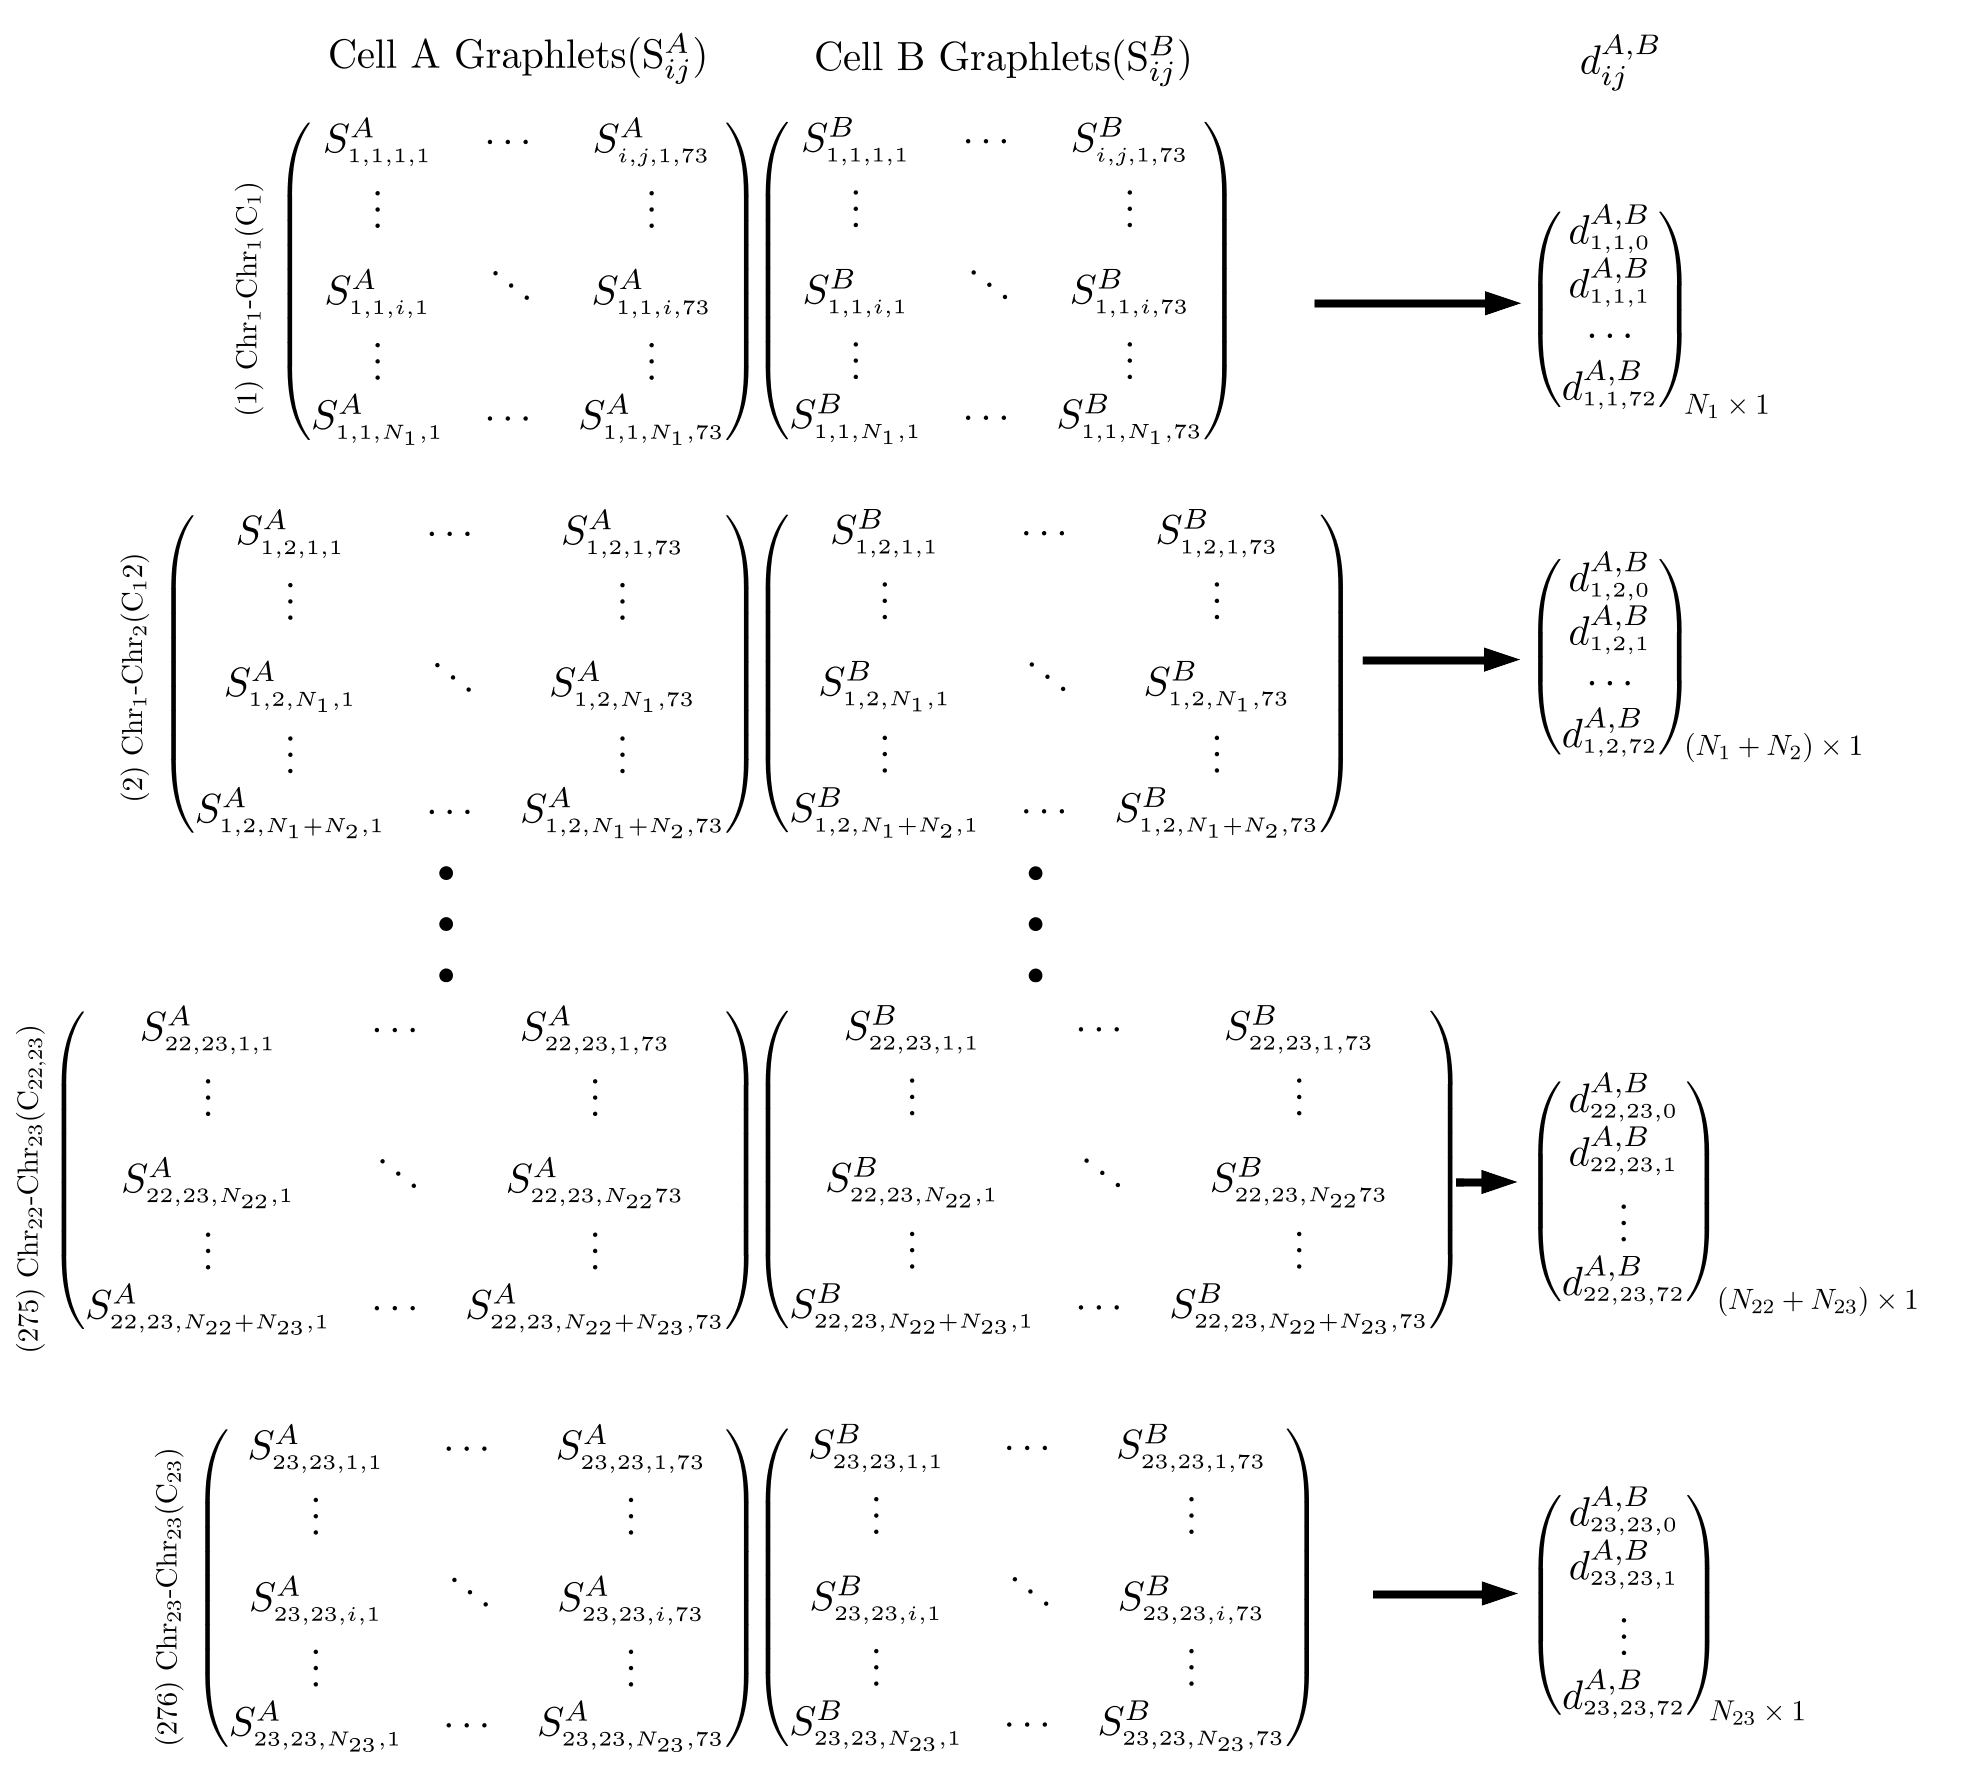
\includegraphics[width=.5\textwidth]{figures/graphlet_distance_schema.png}
    \caption{Calculating pair-wise loci distances. For each loci (row) 
    in each
    contact map in MIT cell line, its distance is calculated based on
    equation \ref{eq:distance_total} with the corresponding loci in
    leukemic cells. The result of this process is a 
    \textit{signature distance vector} of size
    $|V^{ij}| = N_i+N_j$ for each contact map.
    }
    \label{graphlet_distance_schema}
\end{figure}
\begin{figure}
    \centering
    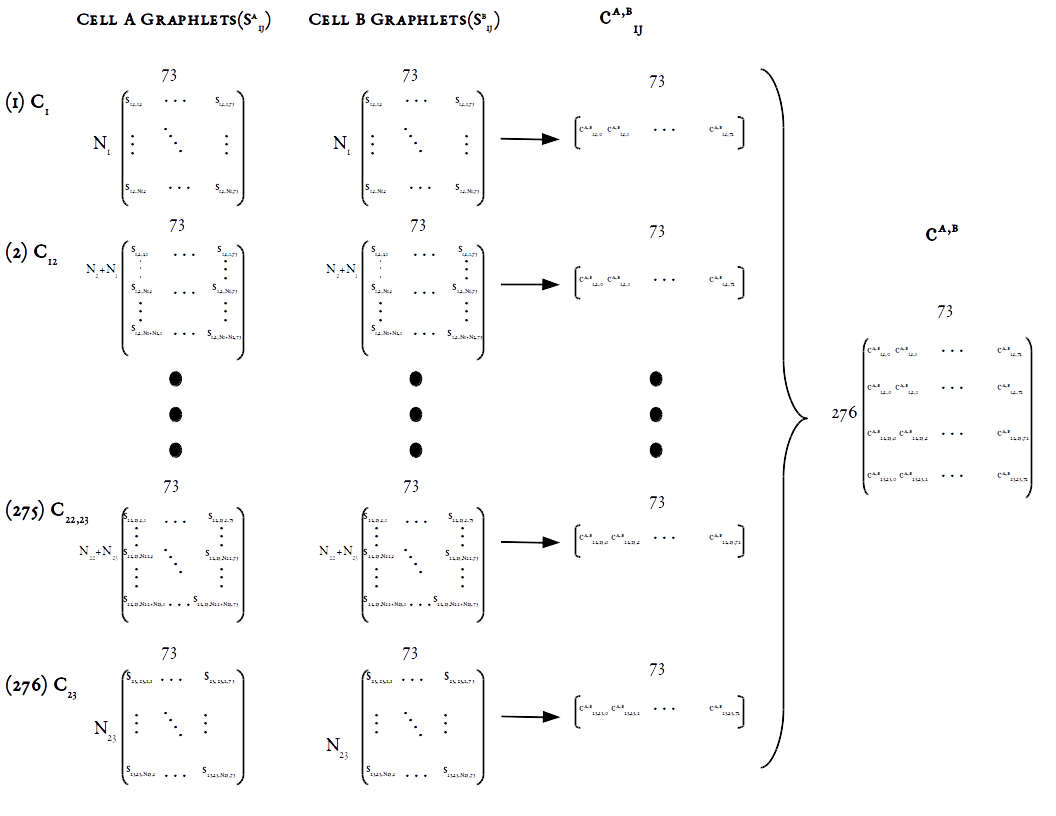
\includegraphics[width=.5\textwidth]{figures/graphlet_correlation_schema.png}
    \caption{Calulating pair-wise orbit correlations. For each orbit (column)
    in each contact map in MIT cell line, its correlation with the
    same orbit in the same contact map 
    in leukemic cells is calculated. The result of
    this process is a \textit{signature correlation} vector of size
    73 which captures how similar frequencies of two orbits are.}
    \label{graphlet_correlation_schema}
\end{figure}
%$
%\begin{pmatrix}
%    {S}^A_{\scriptscriptstyle i,j,1,1}         &
%    \cdots                                     &    
%    {S}^A_{\scriptscriptstyle i,j,1,72}        \\
%%%%%%%%%%%%%%%%%%%%%%%%%%%%%%%%%%%%%%%%%%%%%%%%%%%%%
%    \vdots                                     &                
%                                               &      
%    \vdots                                     \\
%%%%%%%%%%%%%%%%%%%%%%%%%%%%%%%%%%%%%%%%%%%%%%%%%%%%%
%   {S}^A_{\scriptscriptstyle i,j,N_1,1}    &
%   \ddots                                            &    
%   {S}^A_{\scriptscriptstyle i,j,N_1, 72} \\
%%%%%%%%%%%%%%%%%%%%%%%%%%%%%%%%%%%%%%%%%%%%%%%%%%%%%
%    \vdots                                     &                
%                                               &      
%    \vdots                                     \\
%%%%%%%%%%%%%%%%%%%%%%%%%%%%%%%%%%%%%%%%%%%%%%%%%%%%%
%   {S}^A_{\scriptscriptstyle i,j,N_1+N_2,1}   &
%    \cdots                                &
%   {S}^A_{\scriptscriptstyle i,j,N_1+N_2, 72}
%\end{pmatrix}
%$
%
%$
%\begin{pmatrix}
%    {C}^A_{\scriptscriptstyle i,j,1,1}     &
%    \cdots    &
%    {C}^A_{\scriptscriptstyle i,j,1,N_1} \\
%%%%%%%%%%%%%%%%%%%%%%%%%%%%%%%%%%%%%%%%%%%%%%%%%%%%%
%    \vdots                             &
%    \ddots&
%    \vdots                             \\
%%%%%%%%%%%%%%%%%%%%%%%%%%%%%%%%%%%%%%%%%%%%%%%%%%%%%
%    {C}^A_{\scriptscriptstyle i,j,N_1,1}   &
%    \cdots&                  
%    S^A_{\scriptscriptstyle i,j,N_1, N_1}
%%%%%%%%%%%%%%%%%%%%%%%%%%%%%%%%%%%%%%%%%%%%%%%%%%%%%
%\end{pmatrix}
%$

%We divided the task of graphlet comparison into two parts: first we compare
%graphlets from each contact map in normal cell lines (MIT) with the 
%same contact maps in the other three Leukemic cells. Second we compare 
%contact maps in a similar way but this time only between leukemic cells.
%In the former case, the null hypothesis is that there is no difference
%between contact maps of normal cells and leukemic cells and in the latter
%case, the null hypotheis is that there is no difference between 
%different leukemic cells.

We consider two measures of \textit{difference} when comparing contact
map graphlets across cell lines. 
The first measure is \textit{signature distance vectors} between
each contact map of two cell lines. 
For a pair of cells A and B, let 
$\mathbf{S}^A_{ij}$  and $\mathbf{S}^B_{ij}$ be their
signature matrices. The \textit{signature distance} of
contact map $\mathbf{C}_{i,j}$ between A and B is denoted
by $\mathbf{d}^{\scriptscriptstyle A,B}_{ij}$. $\mathbf{d}^{\scriptscriptstyle A,B}_{ij}$ 
is a vector of size $|V_{i,j}|$
and its elements $d^{\scriptscriptstyle A,B}_{i,j,l}$ are
calculated using the following formula from \cite{prvzulj2007biological}:

\begin{equation}
    d^{\scriptscriptstyle A,B}_{i,j,l} = 
    \frac{1}{73}\sqrt{\sum_{o=0}^{72}{t_{lo}^2}}
    \label{eq:distance_total}
\end{equation}

where elements of $t_{i,j,l,o}$ is the
distance between each
loci (row) $l$ in $\mathbf{S}^A$ and the the same loci in 
$\mathbf{S}^B$ for
orbit $o$ as is calculated as below:

\begin{equation}
    t_{lo} = w_o \times 
    \frac{log(S_{ijlo}^A+1) - log(S_{ijlo}^B+1)}
    {log(max(S_{ijlo}^A, S_{ijlo}^B) + 2)}
    \label{eq:distance_single}
\end{equation}


This process is illustrated in Figure \ref{graphlet_distance_schema}.
Using this distance measure, we can quantify how two loci are close to
each other in terms of local neighborhood between the two contact maps.

The second measure of comparison that we use captures how 
similar two orbits are in terms of their count 
frequencies across loci between two contact maps. 
Each column in $S_{ij}$ can provide information
regarding the \textit{frequency distribution} of orbits throughout
the contact map $C_{ij}$. 
We can find how similar these distributions are to each other using
correlation measures.
These correlations are denoted by $\mathbf{m}^{\scriptscriptstyle A,B}_{i,j}$ and
can be calculate using
any plausible correlation measure. 
In this study, for each contact map,  we calculated
similarity between orbit distributions using Pearson's r 
correlation, which is computationally efficient.
However, pearson's r might not be able to capture
non-functional relationships between distributions. As a result, we
also used Maximal Information Coefficient (MIC) 
\cite{reshef2011detecting} in order to compare
correlations. MIC calculates mutual information (MI) between two
distributions, but utilizes dynamic programming in order adjust
bin sizes and numbers in order to achieve highest MI.
MIC values between two variables fall between 0 and 1,
with 0 meaning the two variables are completely independent
and 1 meaning one is dependant on the other.
We used both Pearson's r and MIC in order to compare orbit
frequencies. Although results from both approaches were more
or less consistent, MIC showed higher robustness than Pearson's 
r method.

If MIC is used as correlation measure, each element of 
 $\mathbf{c}$ is calculated as below:
\begin{equation}
    m^{\scriptscriptstyle A,B}_{ijo} = MIC(\mathbf{S}^A_{ij.o}, \mathbf{S}^B_{ij.o})
    \label{eq:mic}
\end{equation}
Alternatively, if we use Pearson criterion we would have:
\begin{equation}
    m^{\scriptscriptstyle A,B}_{ijo} = Pearson(\mathbf{S}^A_{ij.o}, \mathbf{S}^B_{ij.o})
    \label{eq:pearson}
\end{equation}

\section{results and discussions}
\subsection{Contact Map Orbit Vector Distance}
\begin{figure}
    \centering
    \begin{subfigure}[b]{.5\textwidth}
        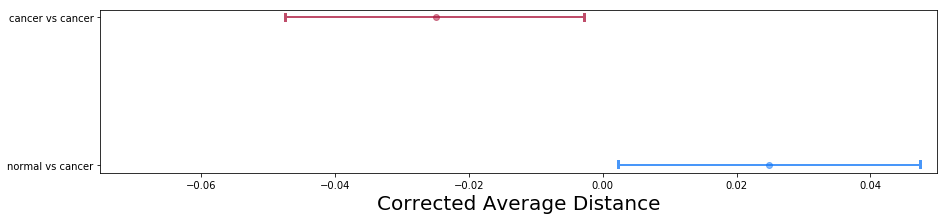
\includegraphics[width=\textwidth]{figures/orbit_distances_normal_vs_cancer.png}
        \caption{}
        \label{fig:orbit_distances_all_a}
    \end{subfigure}

    \begin{subfigure}[b]{.5\textwidth}
        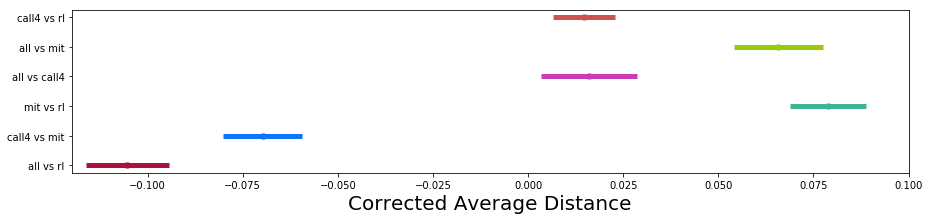
\includegraphics[width=\textwidth]{figures/orbit_distances_cells.png}
        \caption{}
        \label{fig:orbit_distances_all_b}
    \end{subfigure}

    \caption{   
        \textbf{Average Pair-wise graphlet signature difference 
        over all 276 contact maps:}
        Each point on a graph is the result of averaging all
        the distances across all loci of all contact maps for 
        each pair of cells. A 0.1 standard deviation error
        bar is also plotted for each point.
        ($\bar{\mathbf{d}}^{\scriptscriptstyle A,B}$).  
     }
    \label{fig:orbit_distances_all}
\end{figure}

\begin{figure}
    \centering
    \begin{subfigure}[b]{.5\textwidth}
        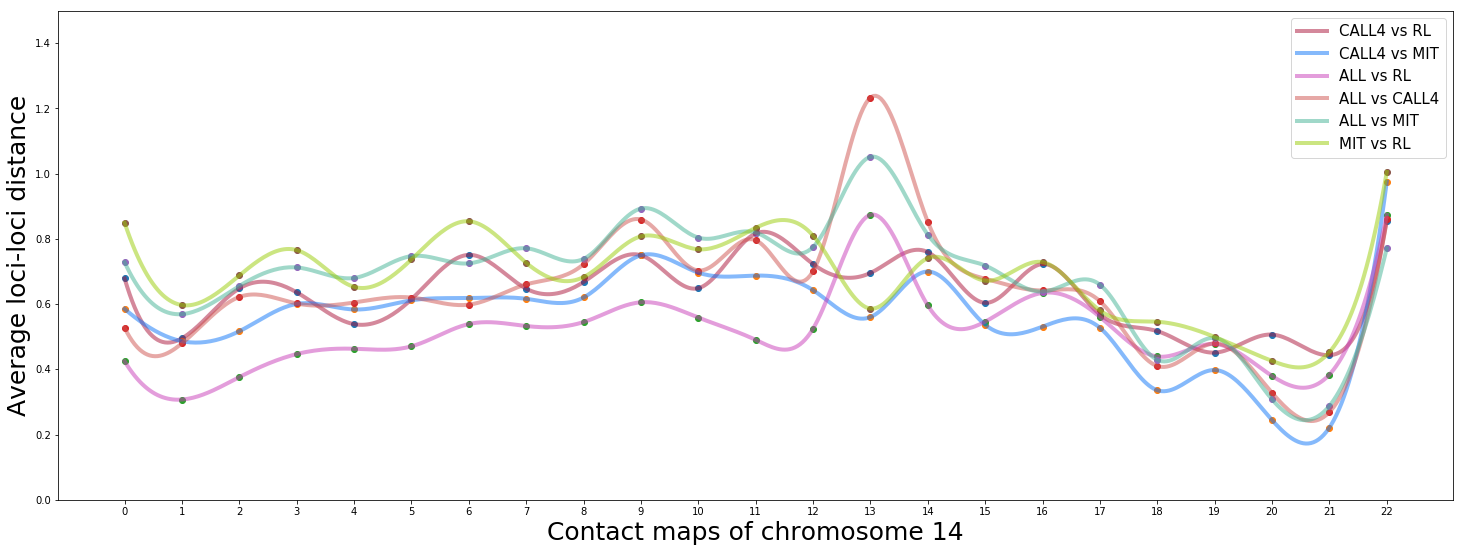
\includegraphics[width=\textwidth]{figures/orbit-distances_chr14.png}
    \end{subfigure}
    \caption{   
        Pair-wise graphlet signature distances for all contact maps of
        chromosome 14. Warm colors as used for cancer-cancer pairs and
        cold colors are used for normal-cancer pairs. As can be seen
        cancer-cancer pairs tend to be close to each other than to the
        normal cell. This is specially true for the first 13 
        inter-chromosomal contact maps.
     }
    \label{fig:orbit_distances_chr14}
\end{figure}


By comparing signature distance vectors, one can find
how contact maps
differ from each other in terms of local structure. 
Contact maps can serve as measures of spatial proximity between
loci. Graphlets capture certain patterns of interaction, or
in other words, spatial neighborhood for each loci. Thus, if
signature vectors of two loci are close,
 it can be inferred that they have 
similar spatial neighborhood.

We can compare pairs of contact maps in terms of their closeness
to each other. 
As an example, in figure
\ref{fig:orbit_distances_chr14}, all pairs of cells are
compared to each other in terms of their distance for contact
maps involving chromosome 14. We can se that 
for the first 13 inter-chromosomal 
contact maps, ALL and RL cell lines are closer to each other
than to other cell lines.

We performed one-way ANOVA statistical test to 
see if there are significant 
difference between cancer-normal and cancer-cancer pairs.
We found that the difference statistically significant difference.
($F(1, 1654) = 20.49, p < 0.0001$).
As illustrated in figure \ref{fig:orbit_distances_all_a},
we can see that normal-cancer pairs have higher distance
from each other than cancer-cancer pairs.

We then continued to investigate each pair separately to
see if there is any significant difference between them.
Again, our statistical tests (ANOVA) showed significant difference
between pairs of cells.
The results are shown in figure \ref{fig:orbit_distances_all_b}.
We can see that ALL-RL pair are closest to each other while
ALL-MIT and MIT-RL are most distant. We found statistcally
significant difference for difference between individual
pairs except for ALL-CALL4 and CALL4-RL as well as
MIT-RL and ALL-MIT. The results of thse tests 
can be found in supplementary material.

The results in figure \ref{fig:orbit_distances_all_b} is also
in keeping with what we see in figure \ref{fig:orbit_distances_chr14}. For example, as mentioned earlier, our results show that
on average, ALL
and RL cell lines are closer to each other than to other
cell lines, which is also the case in figure
\ref{fig:orbit_distances_chr14} for majority of contact maps.

\subsection{MIC Comparison}

\begin{figure*}
    \centering
%    \begin{subfigure}[b]{\textwidth}
%        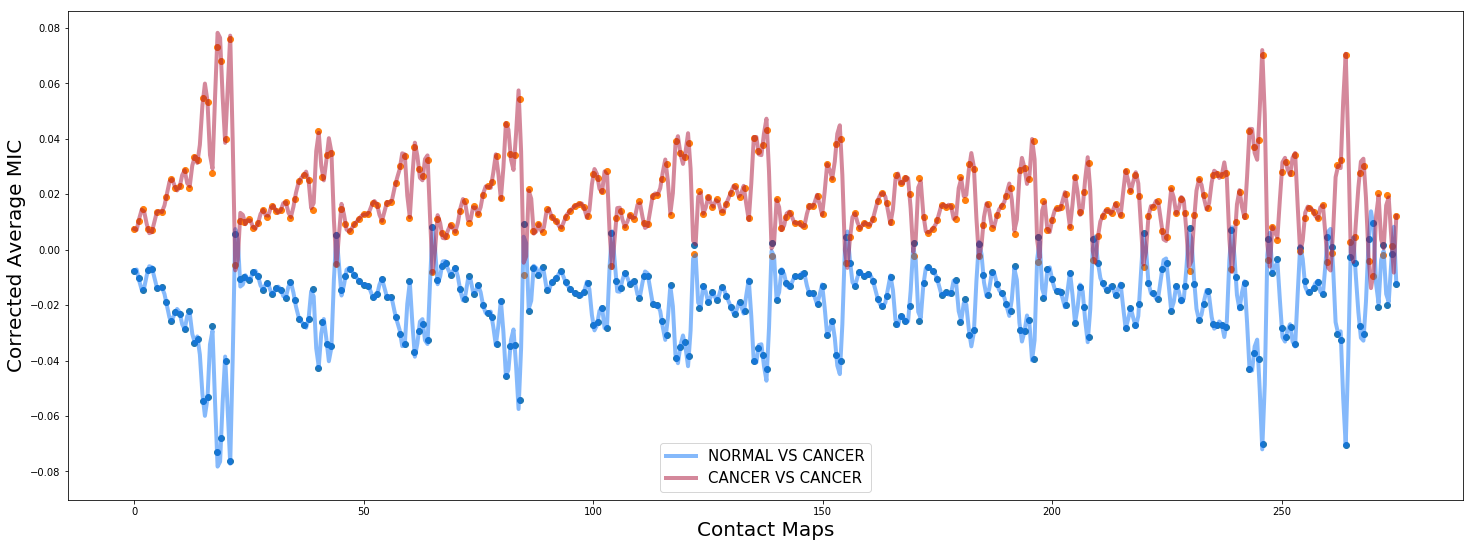
\includegraphics[width=\textwidth]{figures/contact_maps_correlations_cancer_vs_normal.png}
%    \caption{}
%    \label{fig:contact_map_correlations_all}
%    \end{subfigure}

    \begin{subfigure}[b]{\textwidth}
        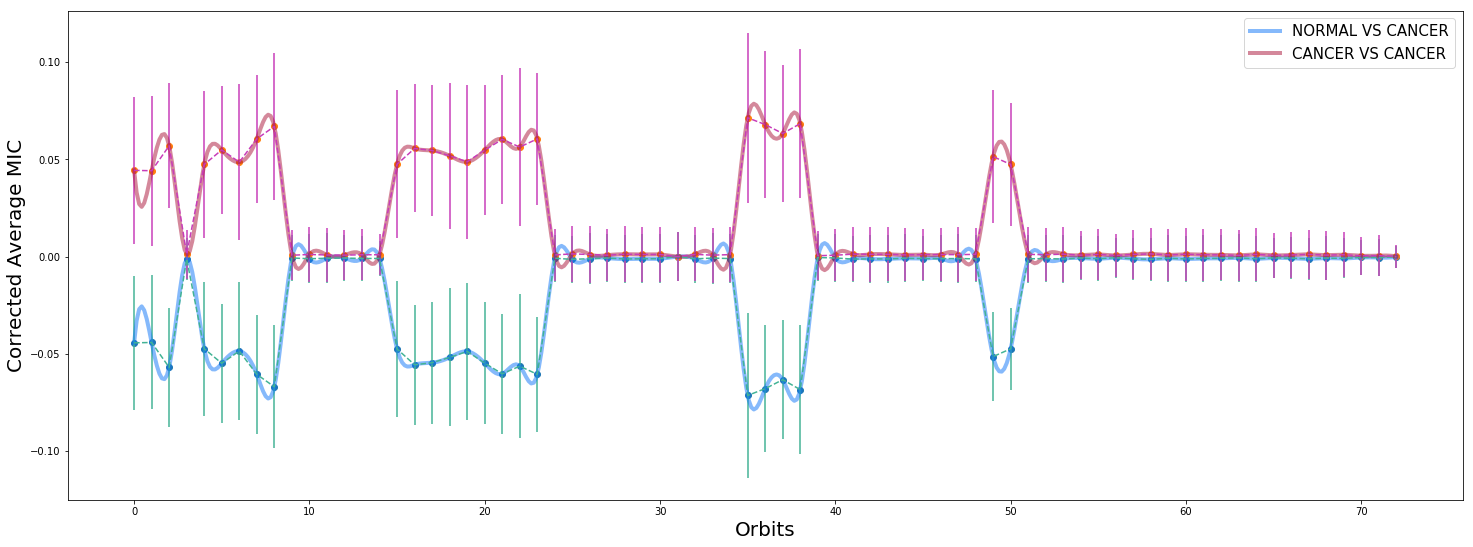
\includegraphics[width=\textwidth]{figures/orbits_correlations_cancer_vs_normal.png}
    \caption{}
    \label{fig:orbits_correlations_normal_vs_cancer}
    \end{subfigure}
    \begin{subfigure}[b]{\textwidth}
    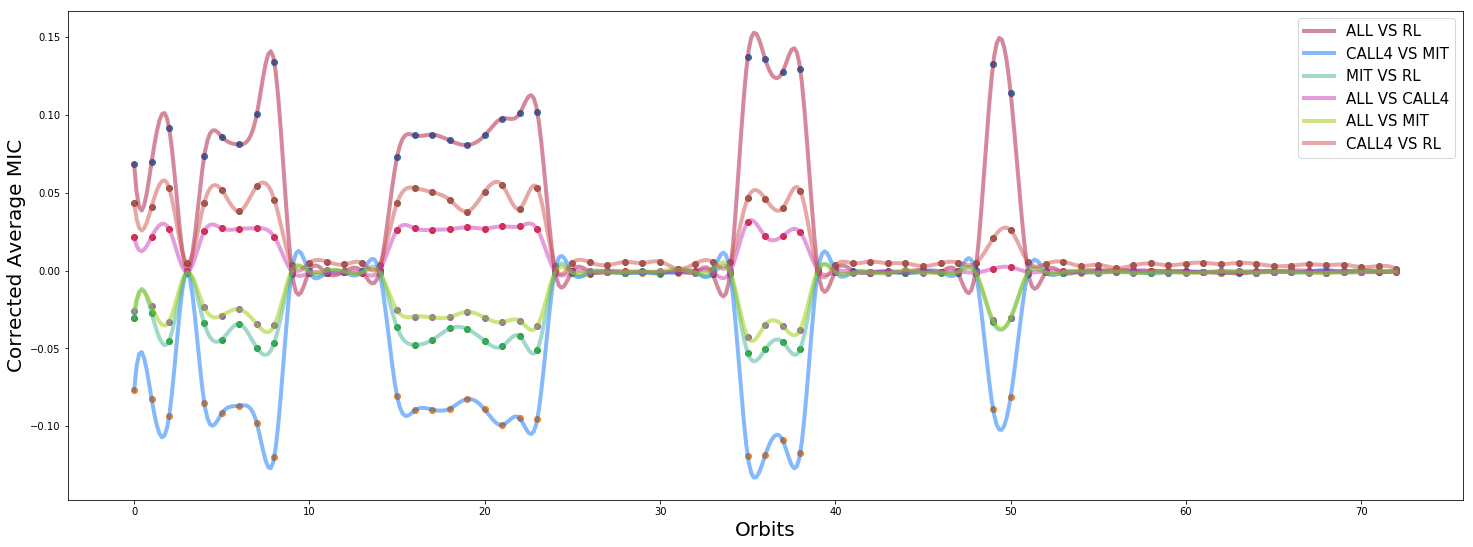
\includegraphics[width=\textwidth]{figures/orbits_correlations_all.png}
    \caption{}
    \label{fig:orbits_correlations_all}
    \end{subfigure}
    \caption{
        \textbf{Pair-wise 
        average contact map orbit correlations
        for all contact maps:}
        ($\bar{\mathbf{m}}^{\scriptscriptstyle \scriptscriptstyle A,B}_{i,j} 
        \quad \forall i,j \in \{1 ... 23\} \quad \& \quad j \ge i$:
        average along the 
        red \textit{vertical} arrow in figure 
        \ref{graphlet_correlation_schema}).
        These values are calculated by averaging over 
        pairwise correlations of orbits of
        $\mathbb{Q}$ in a contact map.
        \textbf{Pair-wise average orbit correlations:}
        In figure \ref{fig:orbits_correlations_all}, each point
        in the graph is the result of averaging pair-wise
        orbit correlations over all contact maps
        ($\frac{1}{276}\sum_{i=0}^{23}\sum_{j=i}^{23}{
        m^{\scriptscriptstyle \scriptscriptstyle A,B}_{i,j, o}} \quad 
        \forall o \in \{0, 1, ..., 72\}$:
        average along the red \textit{horizontal} arrows in figure 
        \ref{graphlet_correlation_schema}).
        Counts for certain orbits are always zero in inter-chromosomal
        maps, leading to average value close to zero in 
        Figure \ref{fig:orbits_correlations_all}.
        In this figure, cancer cells data points are depicted
        in warm colors while normal cells are depicted in
        cold colors in increased contrast. As can be seen
        orbit distributions are more similar to each other
        for cancer cells.
    }
    \label{fig:orbits_correlations}
\end{figure*}

In addition to comparing cells in terms of their
orbit distances, we can compare them by measuring how
often certain graphlets occur in their contact maps. By
doing so, we measure the frequency distribution of the spatial
structures represented by orbits in each contact map. In order
to see how closely such structures are distributed, we can
compare contact maps by calculating the correlation between
their orbit distributions. A higher correlation for certain orbits
would mean higher similarity in terms of that particular spatial
structure between the loci involved.

Before going on with the results,
it is worth mentioning that interchromosomal 
thresholded contact maps 
represent
a bipartide graph with the loci from each chromosome 
on one side. Due to this
bipartide nature of the graphs in inter-chromosomal maps,
count of certain orbits is always 0, resulting in
a correlation values of 0 for them as well.
You can see the bias in 
figure \ref{fig:orbits_correlations} where 
average correlations of orbits
$\mathbb{Q} = \{3, 9, 10{\text -}14, 20{\text -}34, 39{\text -}48, 51{\text -}72\}$ 
are close to zero. In fact all correlations
corresponding to these orbits are 0 except for the ones between 
the same 
chromosomes.

We caclulated pair-wise MIC values 
for each orbit in each of the 276
contact maps from MIT, ALL, RL, and CALL4 data separately. 
We found statistically significant difference between
cancer-cancer and normal-cancer correlations.
($F(73, 1582)=6.29$, $p < 0.00001$, Wilk's $\Lambda = 0.775$)
 The difference  is also illustrated in figure
\ref{fig:orbits_correlations_normal_vs_cancer},
which plots corrected
mean difference of MIC values for cance-cancer and 
normal-cancer correlations.  
We performed statistical test to see if there is a 
significant difference correlation between individual pairs
of cells. Figure \ref{fig:orbits_correlations_all} demonstrate
such difference.
Average correlation over all contac maps
for normal-cancer pairs are smaller
than cancer-cancer pairs. This is corroborated
by the results of statical test which verify that such difference
is in fact signifcant.($F(365, 7882) = 3.91$, $p < 0.00001$, 
Wilk's $\Lambda = 0456$)
Figures \ref{fig:orbits_correlations_normal_vs_cancer} and
\ref{fig:orbits_correlations_all} both show more details about
this difference in correlation. As can be observed, for obits
in $\mathbb{Q}$, normal correlations are smaller than cancer
correlations, while for the rest of the orbits, there is no
difference.

Figure \ref{fig:orbits_correlations} demonstrates that certain
orbits of Leukemic cells
have higher correlation to each other 
than to the
normal MIT cell. In fact our statistical analysis shows that 
\textit {for orbits NOT in $\mathbb{Q}$, 
intra-leukemic orbit correlations are significantly higher
than leukemic-normal orbit correlations}. This implies
there are significant differences between normal and
leukemic cells in terms of their local structure.


\section{Resources}
\textbf{Hi-C Datasets:}
\begin{enumerate}
    \item \href{https://github.com/rasoolianbehnam/watson}{Code base for this article}
    \item \href{http://sysbio.rnet.missouri.edu/T0510/tmp_download/link_to_download_genome_data/}
        {Datasets including cancerous cells}
    \item \href{https://bcm.app.box.com/v/aidenlab/folder/11234760671}{Original Datasets}
\end{enumerate}

\bibliography{lit}
\bibliographystyle{unsrt}
\end{document}
